\part{Introduction}
\section{Introduction}

\begin{frame}
	\partpage
\end{frame}

%%%%%%%%%%%%%%%%%%%%%%%%%%%%%%%%%%%%%%%%%%%%%%%%%%%%%%%%%%%%%%%%%%%%%%%%%%%%%%%
\begin{frame}
	\frametitle{SSH}
	
	\textbf{S}ecure \textbf{Sh}ell, protocol for secure remote login and other secure network services over an insecure network. 
	
	\smallskip
	
	\begin{center}    
  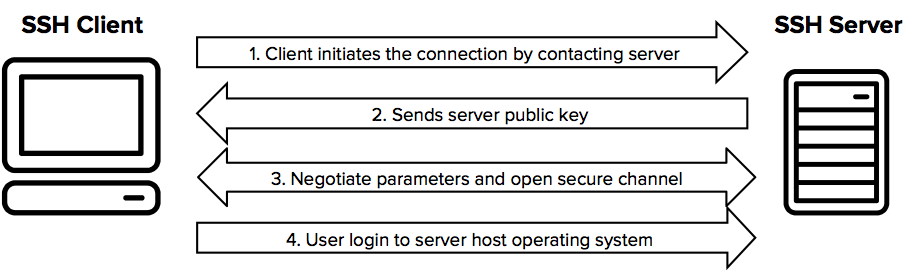
\includegraphics[width=0.7\textwidth]{images/ssh}
  \captionof{figure}{Simplified setup flow (source: ssh.com)}
  \end{center}

	\smallskip
	
	Developed in 1995 in response to a hacking incident, today standard protocol for secure operations.


\end{frame}
%%%%%%%%%%%%%%%%%%%%%%%%%%%%%%%%%%%%%%%%%%%%%%%%%%%%%%%%%%%%%%%%%%%%%%%%%%%%%%%


%%%%%%%%%%%%%%%%%%%%%%%%%%%%%%%%%%%%%%%%%%%%%%%%%%%%%%%%%%%%%%%%%%%%%%%%%%%%%%%
\begin{frame}
	\frametitle{OpenSSH suite}
		
	Suite of secure networking utilities based on SSH protocol.
	
	\medskip
	
	Coming by default in a large number of operating systems
	
	\medskip
		
	Utilities:
	
	\begin{itemize}
	  \item \textsc{scp}, secure copy of files between two different hosts
	  \item \textsc{sftp}, secure file transfer program
	  \item \textsc{ssh}, secure shell client
	  \item \textsc{sshd}, ssh server daemon
	  \item keys utilities (\textsc{ssh-add}, \textsc{ssh-agent}, \textsc{ssh-keygen}, \textsc{ssh-keyscan})
	\end{itemize}

\end{frame}
%%%%%%%%%%%%%%%%%%%%%%%%%%%%%%%%%%%%%%%%%%%%%%%%%%%%%%%%%%%%%%%%%%%%%%%%%%%%%%%


%%%%%%%%%%%%%%%%%%%%%%%%%%%%%%%%%%%%%%%%%%%%%%%%%%%%%%%%%%%%%%%%%%%%%%%%%%%%%%%
\begin{frame}
	\frametitle{Operation Windigo}
	
	Large and sophisticated operation started in 2011 and discovered after 3 years.
	
	\smallskip
	
	The operation has compromised linux servers in order to steal SSH credentials, redirect web traffic and send spam message.
	
	\smallskip
	
  Three different components of the operations:
  
  \begin{itemize}
    \item \textbf{Ebury, OpenSSH backdoor} used to gain full access, steal credentials and keep control of the servers.
    \item Cdorked, an HTTP backdoor used to redirect traffic and a modified DNS server to resolve arbitrary IP addresses.
    \item Calfbot, a Perl script used to send spam.
  \end{itemize}	

	\smallskip
	
  Results:
  
  \begin{itemize}
    \item highly portable malicious modules were developed in order to cover as many system as possibile.
    \item 25,000 unique servers compromised.
    \item 500,000 visitors per day redirected to malicious websites.
    \item 35,000,000 spam email sent.
  \end{itemize}
\end{frame}
%%%%%%%%%%%%%%%%%%%%%%%%%%%%%%%%%%%%%%%%%%%%%%%%%%%%%%%%%%%%%%%%%%%%%%%%%%%%%%%

%%%%%%%%%%%%%%%%%%%%%%%%%%%%%%%%%%%%%%%%%%%%%%%%%%%%%%%%%%%%%%%%%%%%%%%%%%%%%%%
\begin{frame}
	\frametitle{Post-operation analysis}
	
	Post-operation analysis lead ESET to extend coverage about OpenSSH backdoors.
	
	\smallskip

	After months of research and data collection, ESET grouped a series of samples in 21 different OpenSSH malware families, 12 of them undocumented at the time of the paper. 
	
	\begin{center}    
  
\includegraphics[width=0.5\textwidth]{images/eset-logo}
  \captionof{figure}{ESET - IT security company}
  \end{center}

	\smallskip

  Malware were divided according to common features and cataloged by complexity and time of activity.  
	
\end{frame}
%%%%%%%%%%%%%%%%%%%%%%%%%%%%%%%%%%%%%%%%%%%%%%%%%%%%%%%%%%%%%%%%%%%%%%%%%%%%%%%

